\documentclass{beamer}

\mode<presentation> {
\usetheme{CambridgeUS}
\usecolortheme{seagull}
\usefonttheme{default}
}

\usepackage{graphicx}
\usepackage{booktabs}
\usepackage{ragged2e}
\usepackage{minted}
\usepackage{lipsum}
\usepackage[export]{adjustbox}

%----------------------------------------------------------------------------------------
%	My Customized Settings
%----------------------------------------------------------------------------------------

\definecolor{UniBlue}{RGB}{83,121,170}
\definecolor{DarkGray}{RGB}{90,90,90}
\definecolor{LightGray}{RGB}{150,150,150}
\definecolor{TextGreen}{RGB}{115,155,15}
\definecolor{Ocean}{RGB}{23,142,189}
\definecolor{BG}{RGB}{215,215,215}


\setbeamercolor{normal}{fg=DarkGray}
\setbeamercolor{title}{fg=UniBlue}
\setbeamercolor{frametitle}{fg=UniBlue}
\setbeamercolor{structure}{fg=UniBlue}
\setbeamercolor{normal text}{fg=DarkGray,bg=white}
\setbeamercolor{section number projected}{bg=UniBlue,fg=white}

\setbeamertemplate{itemize item}{\scriptsize\raise1.25pt\hbox{\donotcoloroutermaths$\blacktriangleright$}}
\setbeamertemplate{itemize subitem}{\tiny\raise1.5pt\hbox{\donotcoloroutermaths$\bullet$}}
\setbeamertemplate{itemize subsubitem}{\tiny\raise1.5pt\hbox{\donotcoloroutermaths$\blacksqaure$}}
\setbeamercolor{itemize item}{fg=darkred}
\setbeamercolor{itemize subitem}{fg=TextGreen}
\setbeamercolor{itemize subbody}{fg=LightGray}

\setbeamertemplate{enumerate subitem}{\insertenumlabel.\insertsubenumlabel}
\setbeamertemplate{enumerate subsubitem}{\insertenumlabel.\insertsubenumlabel.\insertsubsubenumlabel}
\setbeamertemplate{enumerate mini template}{\insertenumlabel}

\setbeamertemplate{navigation symbols}{}

\newcommand\VeryLargeFont{\fontsize{30}{15}\selectfont}
\newcommand\LargeFont{\fontsize{15}{15}\selectfont}
\newcommand\TinyFont{\fontsize{6}{6}\selectfont}

\setbeamertemplate{frametitle} {
  \nointerlineskip
  \begin{beamercolorbox}[sep=0.15cm,ht=1.3em,wd=\paperwidth]{frametitle}
    \vbox{}\vskip-2ex
    \strut\insertframetitle\strut
    \vskip-0.8ex
  \end{beamercolorbox}
}

\defbeamertemplate*{title page}{customized}[1][] {
  \centering
  \bigskip
  \bigskip
  \bigskip
  \usebeamercolor[fg]{title}\insertsubtitle\par
  \usebeamerfont{title}\inserttitle\par
  \usebeamerfont{subtitle}
  \bigskip
  \usebeamercolor[fg]{normal}
  \usebeamerfont{author}\insertauthor\par
  \usebeamerfont{institute}\insertinstitute\par
  \usebeamerfont{date}\insertdate\par
  \bigskip
  \bigskip
  \bigskip
  \bigskip
  \bigskip
  \usebeamercolor[fg]{titlegraphic}\inserttitlegraphic
}

%----------------------------------------------------------------------------------------
%	TITLE PAGE
%----------------------------------------------------------------------------------------
\title[Introduction]{An Introduction to Python}
\author{Parham Alvani}
\institute[AUT] {
  Amirkabir University of Technology \\
  \medskip
  {\small\tt parham.alvani@gmail.com}
}
\date{May 15, 2015}
\titlegraphic{\hspace*{5cm}
\includegraphics[width=2cm]{figs/aut_logo.jpeg}}

\begin{document}

\begin{frame}
\titlepage
\end{frame}

%----------------------------------------------------------------------------------------
%	PRESENTATION SLIDES
%----------------------------------------------------------------------------------------

%------------------------------------------------
\section{}
\subsection{}

%------------------------------------------------
\begin{frame}[fragile]
	\frametitle{Keyboard Input}
	\begin{columns}[c]
		\begin{column}{30cm}
			\vspace{.1cm}
			\begin{itemize}
				\item The input() function reads a line from sys.stdin and \\
				 returns it with the trailing newline stripped.
			\end{itemize}
			\begin{scriptsize}
				\begin{minted}[
				bgcolor=BG,
				frame=lines,
				framesep=2mm,
				baselinestretch=1.2,
				linenos]
				{python}
				name = input("Enter your input: ");
				print("Received input is : ", name)
				\end{minted}
			\end{scriptsize}
		\end{column}
	\end{columns}
\end{frame}

%------------------------------------------------
\begin{frame}
	\frametitle{Lists}
	\begin{columns}[c]
		\begin{column}{30cm}
			\vspace{.1cm}
			\begin{itemize}
				\justifying
				\item The most basic data structure in Python is the sequence.
				\item Each element of a sequence is assigned a number - its position or index.
				\item The first index is zero, the second index is one, and so forth.
			\end{itemize}
		\end{column}
	\end{columns}
	\vspace{.5cm}
	\hspace*{5.5cm} 
\includegraphics[width=5cm]{figs/list.jpg}	
\end{frame}

%------------------------------------------------
\begin{frame}
	\frametitle{Tuples}
	\begin{columns}[c]
		\begin{column}{30cm}
			\vspace{.05cm}
			\begin{itemize}
				\justifying
				\item A tuple is a sequence of immutable Python objects.
				\item Tuples are sequences, just like lists.
				\item The differences between tuples and lists are:
				\begin{itemize}
						\item the tuples cannot be changed unlike lists
						\item tuples use parentheses, whereas lists use square brackets.
				\end{itemize}
			\end{itemize}
		\end{column}
	\end{columns}
	\vspace{.1cm}
	\hspace*{5.5cm} 
\includegraphics[width=5cm]{figs/tuple.jpg}
\end{frame}

%------------------------------------------------
\begin{frame}
	\frametitle{Dictionary}
	\begin{columns}[c]
		\begin{column}{30cm}
			\vspace{.1cm}
			\begin{itemize}
				\justifying
				\item Each key is separated from its value by a colon (:)
				\item The items are separated by commas
				\item The whole thing is enclosed in curly braces.
			\end{itemize}
		\end{column}
	\end{columns}
	\vspace{.5cm}
	\hspace*{5.5cm} 
\includegraphics[width=5cm]{figs/dictionary.jpg}
\end{frame}

%------------------------------------------------
\begin{frame}
	\frametitle{Flow Control}
	\begin{columns}[c]
		\begin{column}{30cm}
			\vspace{.1cm}
			\begin{itemize}
				\justifying
				\item If-Then-Else
				\item For
				\item While
				\item Exceptions
			\end{itemize}
		\end{column}
	\end{columns}
	\vspace{.5cm}
	\hspace*{5.5cm} 
\includegraphics[width=5cm]{figs/flow-control.jpg}
\end{frame}

%------------------------------------------------
\begin{frame}
	\frametitle{Functions}
	\begin{columns}[c]
		\begin{column}{30cm}
			\vspace{.1cm}
			\begin{itemize}
				\justifying
				\item Function blocks begin with the keyword \textcolor{orange}{def}, \\
				followed by the function name and parentheses.
				\item Any input parameters or arguments should be placed \\
				within these parentheses.
				\item The first statement of a function can be an optional statement - \\
				the documentation string of the function or docstring.
			\end{itemize}
		\end{column}
	\end{columns}
	\vspace{.1cm}
	\hspace*{5cm} 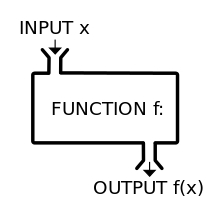
\includegraphics[width=5cm]{figs/functions.jpg}
\end{frame}

%------------------------------------------------
\begin{frame}[fragile]
	\frametitle{Functions}
	\begin{columns}[c]
		\begin{column}{30cm}
			\vspace{.1cm}
			\begin{scriptsize}
			  	\begin{minted}[
			  	bgcolor=BG,
			  	frame=lines,
			  	framesep=2mm,
			  	baselinestretch=1.2,
			  	linenos]
			  	{python}
		  			def square(x):
				  	    return x * x
		  		\end{minted}
		  		\begin{minted}[
		  		bgcolor=BG,
		  		frame=lines,
		  		framesep=2mm,
		  		baselinestretch=1.2,
		  		linenos]
		  		{python}
			  		def hello():
		  			    return "Hello"
			  	\end{minted}
			  	\begin{minted}[
			  	bgcolor=BG,
			  	frame=lines,
			  	framesep=2mm,
			  	baselinestretch=1.2,
			  	linenos]
			  	{python}
			  	def printme( statement ):
			  	    "This prints a passed string into this function"
			  	    print statement
			  	    return
			  	\end{minted}
			\end{scriptsize}
		\end{column}
	\end{columns}
\end{frame}

%------------------------------------------------
\begin{frame}[fragile]
	\frametitle{Lambda}
	\begin{columns}[c]
		\begin{column}{30cm}
			\vspace{.1cm}
			\begin{itemize}
				\justifying
				\item Python supports simple anonymous functions through the lambda form.
				\item The executable body of the lambda must be an expression \\
				and can't be a statement, which is a restriction that limits its utility.
			\end{itemize}
			\begin{scriptsize}
				\begin{minted}[
				bgcolor=BG,
				frame=lines,
				framesep=2mm,
				baselinestretch=1.2,
				linenos]
				{python}
				foo = lambda x: x * x
				\end{minted}
			\end{scriptsize}
		\end{column}
	\end{columns}
	\vspace{.1cm}
	\hspace*{5cm} 
\includegraphics[width=5cm]{figs/lambda.png}
\end{frame}

%------------------------------------------------
\begin{frame}
	\frametitle{Classes}
	\begin{columns}[c]
		\begin{column}{30cm}
			\vspace{.1cm}
			\begin{itemize}
				\justifying
				\item The class statement creates a new class definition.
				\item The name of the class immediately follows the keyword \textcolor{orange}{class} \\
				followed by a colon as follows
			\end{itemize}
		\end{column}
	\end{columns}
	\vspace{.5cm}
	\hspace*{5.5cm} 
\includegraphics[width=5cm]{figs/class.jpg}
\end{frame}

%------------------------------------------------
\begin{frame}[fragile]
	\frametitle{Classes}
	\begin{columns}[c]
		\begin{column}{30cm}
			\vspace{.05cm}
			\begin{scriptsize}
				\begin{minted}[
				bgcolor=BG,
				frame=lines,
				framesep=2mm,
				baselinestretch=1.2,
				linenos]
				{python}
				class Employee:
				    """
				    Common base class for all employees
				    """
				    empCount = 0
				
				    def __init__(self, name, salary):
				        self.name = name
				        self.salary = salary
				        Employee.empCount += 1
				
				    def displayCount(self):
				        print "Total Employee %d" % Employee.empCount
				
				    def displayEmployee(self):
				        print "Name : ", self.name,  ", Salary: ", self.salary
				\end{minted}
				\begin{minted}[
				bgcolor=BG,
				frame=lines,
				framesep=2mm,
				baselinestretch=1.2,
				linenos]
				{python}
				emp1 = Employee("Zara", 2000)
				\end{minted}
			\end{scriptsize}
		\end{column}
	\end{columns}
\end{frame}

%------------------------------------------------
\begin{frame}
	\frametitle{Garbage Collection}
	\begin{columns}[c]
		\begin{column}{30cm}
			\vspace{.1cm}
			\begin{itemize}
				\justifying
				\item Python deletes unneeded objects automatically to free the memory space.
			\end{itemize}
		\end{column}
	\end{columns}
	\vspace{.5cm}
	\hspace*{5.5cm} 
\includegraphics[width=5cm]{figs/garbage.jpg}
\end{frame}

%------------------------------------------------
\begin{frame}
	\frametitle{Inheritance}
	\begin{columns}[c]
		\begin{column}{30cm}
			\vspace{.1cm}
			\begin{itemize}
				\justifying
				\item Instead of starting from scratch, you can create a class by deriving it \\
				from a preexisting class by listing the parent class in parentheses \\
				after the new class name.
			\end{itemize}
		\end{column}
	\end{columns}
	\vspace{.5cm}
	\hspace*{5.5cm} 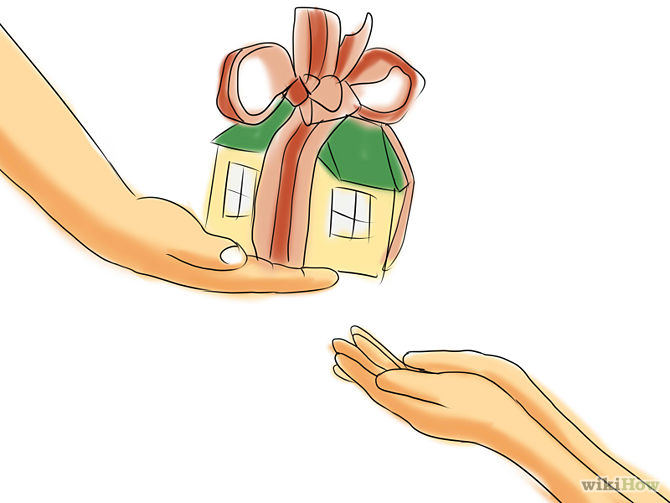
\includegraphics[width=5cm]{figs/Inheritance.jpg}
\end{frame}

%------------------------------------------------
\begin{frame}[fragile]
	\frametitle{Inheritance}
	\begin{columns}[c]
		\begin{column}{30cm}
			\vspace{.05cm}
			\begin{scriptsize}
				\begin{minted}[
				bgcolor=BG,
				frame=lines,
				framesep=2mm,
				baselinestretch=1.2,
				linenos]
				{python}
				class SubClassName (ParentClass1[, ParentClass2, ...]):
				    """
				    Optional class documentation string
				    """
				    # class_suite
				\end{minted}
			\end{scriptsize}
		\end{column}
	\end{columns}
\end{frame}

%------------------------------------------------
\begin{frame}
	\frametitle{Base Overloading Methods}
	\begin{columns}[c]
		\begin{column}{30cm}
			\vspace{.1cm}
			\begin{itemize}
				\justifying
				\item \_\_init\_\_( self [,args...] ) : \textcolor{Ocean}{Constructor (with any optional arguments)}
				\item \_\_del\_\_( self ) : \textcolor{Ocean}{Destructor, deletes an object}
				\item \_\_repr\_\_( self ) : \textcolor{Ocean}{Evaluatable string representation}
				\item \_\_str\_\_( self ) : \textcolor{Ocean}{Printable string representation}
				\item \_\_lt\_\_( self, other ):
				\item \_\_le\_\_( self, other ):
				\item \_\_eq\_\_( self, other ):
				\item \_\_ne\_\_( self, other ):
				\item \_\_gt\_\_( self, other ):
				\item \_\_ge\_\_( self, other ): \\
				\textcolor{Ocean}{These are the so-called “rich comparison” methods,} \\
				\textcolor{Ocean}{and are called for comparison operators in preference to \_\_cmp\_\_() below.}
			\end{itemize}
		\end{column}
	\end{columns}
\end{frame}

%------------------------------------------------
\begin{frame}
	\frametitle{Base Overloading Methods}
	\begin{columns}[c]
		\begin{column}{30cm}
			\vspace{.1cm}
			\begin{itemize}
				\justifying
				\item \_\_cmp\_\_ ( self, x ) : \textcolor{Ocean}{Called by comparison operations if rich comparison} \\
				\textcolor{Ocean}{is not defined.} 
				\item \_\_add\_\_( self, other ):
				\item \_\_sub\_\_( self, other ):
				\item \_\_mul\_\_( self, other ):
				\item \_\_floordiv\_\_( self, other ):
				\item \_\_mod\_\_( self, other ):
				\item \_\_divmod\_\_( self, other ):
				\item \_\_pow\_\_( self, other[, modulo] ):
				\end{itemize}
		\end{column}
	\end{columns}
\end{frame}

%------------------------------------------------
\begin{frame}
	\frametitle{Base Overloading Methods}
	\begin{columns}[c]
		\begin{column}{30cm}
			\vspace{.1cm}
			\begin{itemize}
				\justifying
				\item \_\_lshift\_\_( self, other ):
				\item \_\_rshift\_\_( self, other ):
				\item \_\_and\_\_( self, other ):
				\item \_\_xor\_\_( self, other ):
				\item \_\_or\_\_( self, other ): \\
				\textcolor{Ocean}{These methods are called to implement the binary arithmetic operations} \\
				\textcolor{green}{+, -, *, //, \%, divmod(), pow(), **, \textless\textless, \textgreater\textgreater,
				\&, \textasciicircum, \textbar}
			\end{itemize}
		\end{column}
	\end{columns}
\end{frame}

%------------------------------------------------
\begin{frame}
	\frametitle{Data Hiding}
	\begin{columns}[c]
		\begin{column}{30cm}
			\vspace{.1cm}
			\begin{itemize}
				\justifying
				\item An object's attributes may or may not be visible outside \\
				the class definition.
				\item You need to name attributes with a double underscore prefix, and those \\
				attributes then are not be directly visible to outsiders.
				\item Python protects those members by internally changing the name to \\
				include the class name.
				\item You can access such attributes as \textcolor{orange}{object.\_className\_\_attrName}
			\end{itemize}
		\end{column}
	\end{columns}
	\vspace{1cm}
	\hspace*{5.5cm}
\end{frame}

%------------------------------------------------
\begin{frame}[fragile]
	\frametitle{Data Hiding}
	\begin{columns}[c]
		\begin{column}{30cm}
			\vspace{.05cm}
			\begin{scriptsize}
				\begin{minted}[
				bgcolor=BG,
				frame=lines,
				framesep=2mm,
				baselinestretch=1.2,
				linenos]
				{python}
				#!/usr/bin/python
				
				class JustCounter:
				    __secretCount = 0
				
				    def count(self):
				        self.__secretCount += 1
				        print self.__secretCount
				
				counter = JustCounter()
				counter.count()
				counter.count()
				print counter.__secretCount
				\end{minted}
			\end{scriptsize}
		\end{column}
	\end{columns}
\end{frame}

%------------------------------------------------
\begin{frame}[fragile]
	\frametitle{Data Hiding}
	\begin{columns}[c]
		\begin{column}{30cm}
			\vspace{.05cm}
			\begin{scriptsize}
				\begin{minted}[
				bgcolor=BG,
				frame=lines,
				framesep=2mm,
				baselinestretch=1.2,
				linenos]
				{python}
				1
				2
				Traceback (most recent call last):
				File "test.py", line 12, in <module>
				print counter.__secretCount
				AttributeError: JustCounter instance has no attribute '__secretCount'
				\end{minted}
			\end{scriptsize}
		\end{column}
	\end{columns}
\end{frame}

%------------------------------------------------
\begin{frame}
	\frametitle{What is a metaclass in Python?}
	\begin{columns}[c]
		\begin{column}{30cm}
			\vspace{.1cm}
			\begin{itemize}
				\justifying
				\item A metaclass is the class of a class
				\item Like a class defines how an instance of the class behaves,\\
				 a metaclass defines how a class behaves.
				 \item A class is an instance of a metaclass.
			\end{itemize}
		\end{column}
	\end{columns}
	\vspace{.5cm}
	\hspace*{2cm} 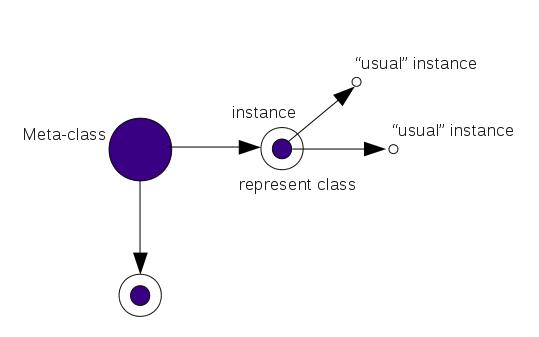
\includegraphics[width=8cm]{figs/meta-class.jpg}
\end{frame}


%------------------------------------------------
\begin{frame}
	\frametitle{Multiple Inheritance}
	\begin{columns}[c]
		\begin{column}{30cm}
			\vspace{.1cm}
			\begin{itemize}
				\justifying
				\item Method Resolution Order (MRO)
				\item C3 Algorithm
			\end{itemize}
		\end{column}
	\end{columns}
	\vspace{1cm}
	\hspace*{5.5cm} 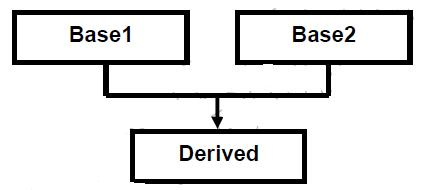
\includegraphics[width=5cm]{figs/multiple-inheritance.jpg}
\end{frame}

%------------------------------------------------
\begin{frame}
	\frametitle{C3 linearization}
	\begin{columns}[c]
		\begin{column}{30cm}
			\vspace{.1cm}
			\begin{itemize}
					\justifying
					\item The C3 superclass linearization is an algorithm used primarily \\
					to obtain the order in which methods should \\
					be inherited (the "linearization") in the presence of \\
					multiple inheritance, and is often termed "MRO" \\
					for Method Resolution Order.	
			\end{itemize}		
		\end{column}
	\end{columns}
\end{frame}

%------------------------------------------------
\begin{frame}[fragile]
	\frametitle{C3 Algorithm}
	\begin{columns}[c]
		\begin{column}{30cm}
			\vspace{.05cm}
			\begin{scriptsize}
				\begin{minted}[
				bgcolor=BG,
				frame=lines,
				framesep=2mm,
				baselinestretch=1.2,
				linenos]
				{text}
				class O
				class A extends O
				class B extends O
				class C extends O
				class D extends O
				class E extends O
				class K1 extends A, B, C
				class K2 extends D, B, E
				class K3 extends D, A
				class Z extends K1, K2, K3
				\end{minted}
			\end{scriptsize}
		\end{column}
	\end{columns}
\end{frame}

%------------------------------------------------
\begin{frame}[fragile]
	\frametitle{C3 Algorithm}
	\begin{columns}[c]
		\begin{column}{30cm}
			\vspace{.05cm}
			\begin{scriptsize}
				\begin{minted}[
				bgcolor=BG,
				frame=lines,
				framesep=2mm,
				baselinestretch=1.2,
				linenos]
				{text}
				L(O)  := [O]                                                     
				
				L(A)  := [A] + merge(L(O), [O])
				= [A] + merge([O], [O])
				= [A, O]                                                  
				
				L(B)  := [B, O]
				L(C)  := [C, O]
				L(D)  := [D, O]
				L(E)  := [E, O]
				
				L(K1) := [K1] + merge(L(A), L(B), L(C), [A, B, C])
				= [K1] + merge([A, O], [B, O], [C, O], [A, B, C])
				= [K1, A] + merge([O], [B, O], [C, O], [B, C])
				= [K1, A, B] + merge([O], [O], [C, O], [C])
				= [K1, A, B, C] + merge([O], [O], [O])
				= [K1, A, B, C, O]
				\end{minted}
			\end{scriptsize}
		\end{column}
	\end{columns}
\end{frame}

%------------------------------------------------
\begin{frame}[fragile]
	\frametitle{C3 Algorithm}
	\begin{columns}[c]
		\begin{column}{30cm}
			\vspace{.05cm}
			\begin{scriptsize}
				\begin{minted}[
					bgcolor=BG,
					frame=lines,
					framesep=2mm,
					baselinestretch=1.2,
					linenos]
					{text}
					L(K2) := [K2] + merge(L(D), L(B), L(E), [D, B, E])
					= [K2] + merge([D, O], [B, O], [E, O], [D, B, E])
					= [K2, D] + merge([O], [B, O], [E, O], [B, E])
					= [K2, D, B] + merge([O], [O], [E, O], [E])
					= [K2, D, B, E] + merge([O], [O], [O])
					= [K2, D, B, E, O]
					
					L(K3) := [K3] + merge(L(D), L(A), [D, A])
					= [K3] + merge([D, O], [A, O], [D, A])
					= [K3, D] + merge([O], [A, O], [A])
					= [K3, D, A] + merge([O], [O])
					= [K3, D, A, O]
				\end{minted}
			\end{scriptsize}
		\end{column}
	\end{columns}
\end{frame}

%------------------------------------------------
\begin{frame}[fragile]
	\frametitle{C3 Algorithm}
	\begin{columns}[c]
		\begin{column}{30cm}
			\vspace{.05cm}
			\begin{scriptsize}
				\begin{minted}[
					bgcolor=BG,
					frame=lines,
					framesep=2mm,
					baselinestretch=1.2,
					linenos]
					{text}
					L(Z)  := [Z] + merge(L(K1), L(K2), L(K3), [K1, K2, K3])
					= [Z] + merge([K1, A, B, C, O], [K2, D, B, E, O], [K3, D, A, O], [K1, K2, K3])
					= [Z, K1] + merge([A, B, C, O], [K2, D, B, E, O], [K3, D, A, O], [K2, K3])
					= [Z, K1, K2] + merge([A, B, C, O], [D, B, E, O], [K3, D, A, O], [K3])
					= [Z, K1, K2, K3] + merge([A, B, C, O], [D, B, E, O], [D, A, O])
					= [Z, K1, K2, K3, D] + merge([A, B, C, O], [B, E, O], [A, O])
					= [Z, K1, K2, K3, D, A] + merge([B, C, O], [B, E, O], [O])
					= [Z, K1, K2, K3, D, A, B] + merge([C, O], [E, O], [O])
					= [Z, K1, K2, K3, D, A, B, C] + merge([O], [E, O], [O])
					= [Z, K1, K2, K3, D, A, B, C, E] + merge([O], [O], [O])
					= [Z, K1, K2, K3, D, A, B, C, E, O]
				\end{minted}
			\end{scriptsize}
		\end{column}
	\end{columns}
\end{frame}

%------------------------------------------------
\begin{frame}[fragile]
	\frametitle{Class method differences in Python}
	\begin{columns}[c]
		\begin{column}{30cm}
			\vspace{.05cm}
			\begin{itemize}
				\justifying
				\item Bound, unbound and static
				\item Basically, a call to a member function a bound function \\
				is translated to a call to an unbound method. 
			\end{itemize}
			\vspace{0.5cm}
			\begin{scriptsize}
				\begin{minted}[
				bgcolor=BG,
				frame=lines,
				framesep=2mm,
				baselinestretch=1.2,
				linenos]
				{python}
				class Test(object):
				    def method_one(self):
				        print "Called method_one"
				
				a_test = Test()
				
				a_test.method_one()
				# is translated to
				Test.method_one(a_test)
				\end{minted}
			\end{scriptsize}
		\end{column}
	\end{columns}
\end{frame}

%------------------------------------------------
\begin{frame}[fragile]
	\frametitle{Class method differences in Python}
	\begin{columns}[c]
		\begin{column}{30cm}
			\vspace{.05cm}
			\begin{itemize}
				\justifying
				\item The @staticmethod tells the built-in default metaclass type \\
				(the class of a class) to not create bound methods for method\_two.
			\end{itemize}
			\vspace{0.5cm}
			\begin{scriptsize}
				\begin{minted}[
				bgcolor=BG,
				frame=lines,
				framesep=2mm,
				baselinestretch=1.2,
				linenos]
				{python}
				class Test(object):
				    @staticmethod
				    def method_two():
				        print "Called method two"
				
				a_test = Test()
				a_test.method_two()
				# is translated to
				Test.method_two()
				\end{minted}
			\end{scriptsize}
		\end{column}
	\end{columns}
\end{frame}

%------------------------------------------------
\begin{frame}
	\vspace{1cm}
	\begin{Huge}
		\begin{center}
			\usebeamercolor[fg]{title}Questions?
		\end{center}
	\end{Huge}
\end{frame}

\end{document} 